%%%%%%%%%%%%%%%%%%%%%%%%%%%%%%%%%%%%%%%%%%%%%%%%%%%%%%%%%%%%%%%%%%%%%%%%%%%%
\section{Supporting Information Appendix} \label{ap_b_abcsal}


%--------------------------------------------------------%
\subsection{C2VSim average annual land surface and rootzone water budget (1961-10-31 to 2001-09-30)}

% 01_mm_plots_tables.R in F:/ ... POst_QE_Research/DISSERTATION/01_mm
% search for gw_and_sw_c table

\bgroup

\renewcommand{\arraystretch}{1.5}

\setlength{\tabcolsep}{1.3em}

% 05_calc_avg_budgets.R 01_mm_plots_tables.R in F:/ ... POst_QE_Research/DISSERTATION/01_mm/code
% M mtons of mass calculated by 264.53*1E12*5.543/1E9/1E6
\centering
\begin{threeparttable}
	\begin{table}[H]
		\caption{C2VSim average annual land surface and rootzone water budget (1961-10-31 to 2001-09-30).}
		
		\begin{tabular}{rlrrrr}
			
			
			
			& \textbf{Source} & $\bm{Q \: \: (km^3/yr)}$ & $\bm{C \: \: (mg/L)}$ & $\bm{m \: \: (Metric \: Mtons)}$ & \\ 
			\hline
			& $P$ & 6.760 & * & * & \\ 
			& $D$ & 5.543 & 264.53 & 1.47 & \\ 
			& $Pt$ & 4.337 & 0 & 0 & \\ 
			& $ET$ & -13.681 & 0 & 0 & \\ 
			& $N$ & -1.883 & * & * & \\ 
			& $Ro$ & -0.400 & 0 & 0 & \\
			& $Rf$ & -0.670 & 0 & 0 & \\
			& $\Delta S$ & 0.006 &  &  & \\ 
			\hline
			\multicolumn{4}{l}{\scriptsize{* non-constant term calculated at each time step}} 
		\end{tabular}
		
		$Q$ is the volumetric flow rate, $C$ is the concentration of TDS, and $m$ is the mass of salt. Land and rootzone budget terms are: 
		$P$ = groundwater pumping, 
		$D$ = surface water diversions,
		$Pt$ = precipitation,
		$ET$ = evapotranspiration,
		$N$ = net deep percolation from vadose zone into groundwater,
		$Ro$ = runoff,
		$Rf$ = return flow,
		$\Delta S$ = change in storage. 
		The water balance equation is: $\Delta S = P + D + Pt - ET - N - Ro - Rf$.  
		
		\label{ap_b_lsb}
	\end{table}
	
\end{threeparttable}


\egroup
\clearpage


%--------------------------------------------------------%
\subsection{TDS of natural waters measured at NWIS stations in Kern, Kings, Tulare, and Fresno counties}


\bgroup

\begin{figure}[H]
	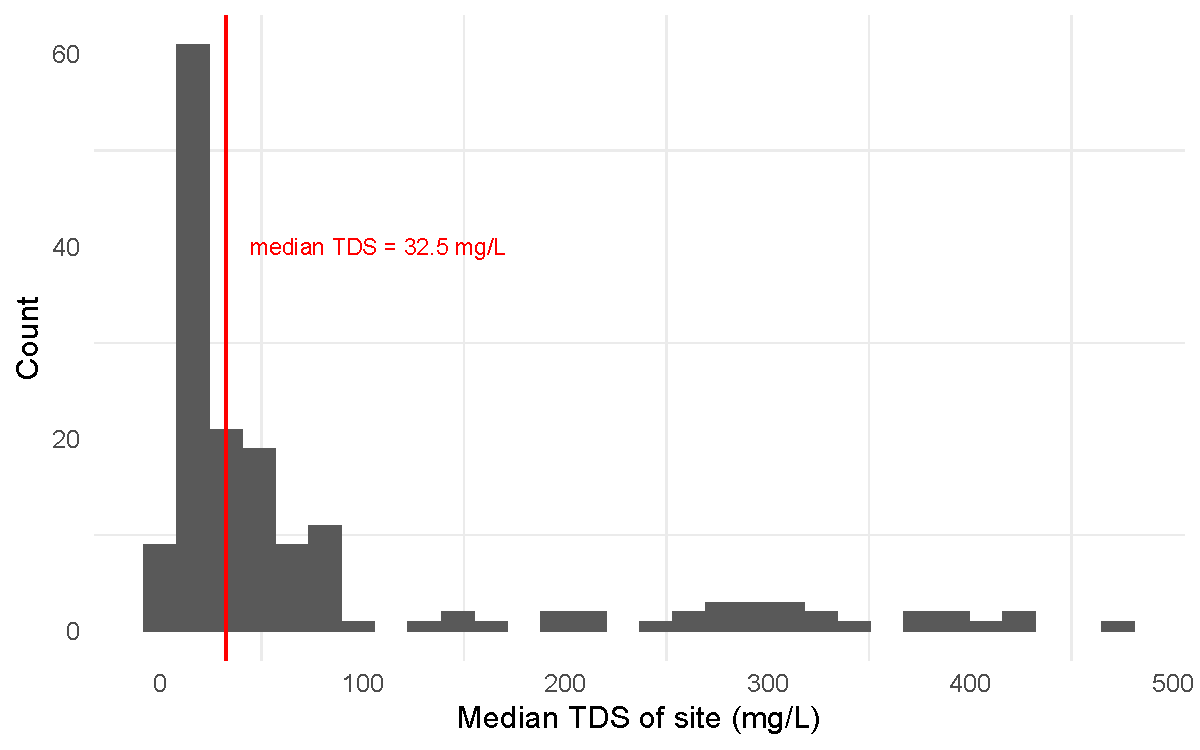
\includegraphics[width=\textwidth]{ch3_appendix_figs/natural_waters.pdf}
	\caption{Median TDS of natural waters measured at NWIS stations in Kern, Kings, Tulare, and Fresno counties*.}
	\label{ap_b_nat_waters}
\end{figure}

\egroup

*the following 162 NWIS station codes were analyzed: USGS-11186000, USGS-11187000, USGS-11191000, USGS-11194000, USGS-11203200, USGS-11203500, USGS-11204900, USGS-11206500, USGS-11206700, USGS-11206800, USGS-11206820, USGS-11208000, USGS-11208605, USGS-11208607, USGS-11208610, USGS-11208615, USGS-11208620, USGS-11208625, USGS-11208630, USGS-11208650, USGS-11208680, USGS-11208715, USGS-11208730, USGS-11209500, USGS-11210500, USGS-11210950, USGS-11212423, USGS-11213500, USGS-11218500, USGS-11220000, USGS-11221500, USGS-11221900, USGS-11222700, USGS-11230540, USGS-11247000, USGS-11250000, USGS-11251000, USGS-11253500, USGS-11254000, USGS-11256000, USGS-345002118424201, USGS-351355119194801, USGS-351745119203401, USGS-352641119404801, USGS-353328119395901, USGS-353933118274800, USGS-353953118234500, USGS-354144118263400, USGS-354251119373101, USGS-354307119351401, USGS-355428119234901, USGS-355802116555201, USGS-360039119583101, USGS-361419119511801, USGS-362100118454001, USGS-362102118241501, USGS-362102118402801, USGS-362243119471001, USGS-362317118245201, USGS-362511118245201, USGS-362540118452901, USGS-362542118432701, USGS-362629118245301, USGS-362647118360801, USGS-362718118244101, USGS-362730118281401, USGS-362730118343001, USGS-362730118400001, USGS-362808118242101, USGS-362808118242102, USGS-362852118240901, USGS-362937118200801, USGS-362947118193801, USGS-363010118302801, USGS-363107118453501, USGS-363112118454601, USGS-363113118480101, USGS-363138118445801, USGS-363310118240101, USGS-363331118450701, USGS-363438118243901, USGS-363455118251301, USGS-363616118245801, USGS-363623118441401, USGS-363629118424201, USGS-363634118444901, USGS-363820118253101, USGS-363911118315501, USGS-363922119402001, USGS-364000118404500, USGS-364019120321101, USGS-364101118412400, USGS-364153118344701, USGS-364155119445000, USGS-364155119445002, USGS-364203118345000, USGS-364218118343401, USGS-364234118404401, USGS-364235118345200, USGS-364236118411301, USGS-364247118352200, USGS-364345118345901, USGS-364400120202600, USGS-364406118382200, USGS-364427118373900, USGS-364454118370100, USGS-364510118262301, USGS-364511118260901, USGS-364519120222001, USGS-364646118320301, USGS-364647118321701, USGS-364658118371801, USGS-364659118372100, USGS-364712120230400, USGS-364718120221800, USGS-364723118403401, USGS-364732118360601, USGS-364746119445400, USGS-364754118344801, USGS-364809118413901, USGS-364818119443800, USGS-364818119464700, USGS-365016120261300, USGS-365027120313401, USGS-365035118321501, USGS-365035119555300, USGS-365105120293001, USGS-365130119504200, USGS-365130120265200, USGS-365202118303701, USGS-365226118255801, USGS-365235119465800, USGS-365235119470700, USGS-365238118260101, USGS-365338118320901, USGS-365453118313301, USGS-365543118444001, USGS-365650118403001, USGS-365743118382501, USGS-365808118375901, USGS-365845118373601, USGS-365912120300000, USGS-365922118264801, USGS-365940120300000, USGS-365952118351001, USGS-370000119393000, USGS-370025119414500, USGS-370059118394101, USGS-370102118391901, USGS-370111118344601, USGS-370140119393000, USGS-370312118342201, USGS-370515120321600, USGS-370539118350701, USGS-370555118354601, USGS-370847118462601, USGS-371017118424601, USGS-371025118432101, USGS-371033118423501, USGS-371123118473601, USGS-371127118454201, USGS-371212118480001


\clearpage


% 01_mm_plots_tables.R in F:/ ... POst_QE_Research/DISSERTATION/01_mm
% search for gw_and_sw_c_summary table


\bgroup

\renewcommand{\arraystretch}{1.5}

\begin{table}[H]
	
	\caption{TDS of natural waters (derived from NWIS samples, see Figure \ref{ap_b_nat_waters}) and agricultural diversions (derived from Central Valley Project and State Water Project water and salt budgets). $C$ is the concentration of TDS. From C2VSim, total applied water is 45.1\% agricultural diversions and 54.9\% groundwater pumping. Natural waters are the TDS of $R$, $B$, $C$, $I$, and $M$ in Table 1. Agricultural diversions are $D$ in Table \ref{ap_b_lsb}.}
	\centering
	
	\begin{tabular}{lr}
		
		\textbf{Source} & $\bm{C \: \: (mg/L)}$ \\ 
		\hline
		Natural waters & 32.50 \\ 
		Agricultural diversions & 264.53 \\ 
		\hline
	\end{tabular}
	
	\label{ap_b_gw_and_sw_c_summary}
\end{table}

\egroup



%--------------------------------------------------------%
\subsection{Spatial distribution of pre-1960 groundwater quality in the TLB}

% in F:\Box Sync\Research\Post QE Research\DISSERTATION\01_mm\code\02_reanalyze_gw_tds.R
% search predev_tds_map.pdf

\begin{figure}[H]
	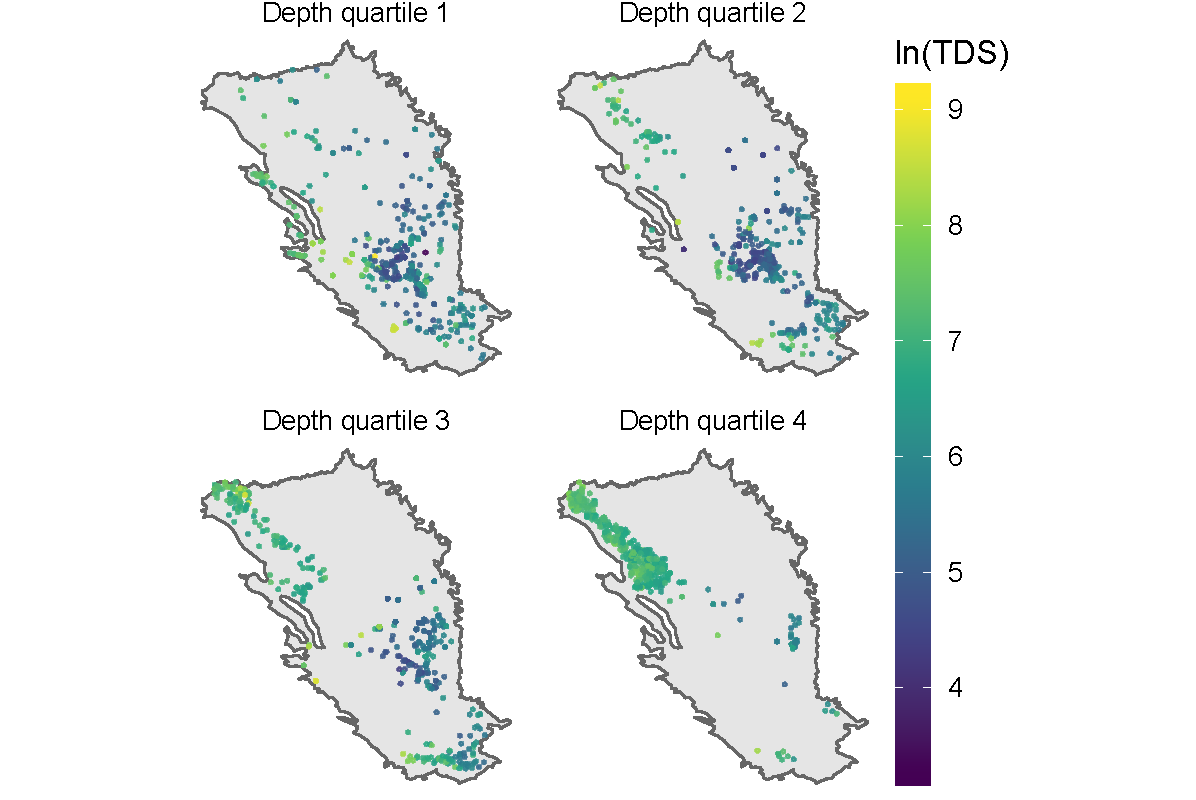
\includegraphics[width=\textwidth]{ch3_appendix_figs/predev_tds_map.pdf}
	\caption{Spatial distribution of pre-1960 groundwater quality (Figure \ref{fig:predev_tds_bc}) at 4 depth quartiles from land surface to 762 m in depth (near the base of fresh water). The mixing model (depth = 212 $m$) is contained within depth quartiles 1 and 2. Quartile 1 = 0.00 to -160.93 $m$, Quartile 2 = -160.94 to -256.03  $m$, Quartile 3 = -256.04 $m$ to -454.15, Quartile 4 = -454.16 to -762.00 $m$.}
	\label{ap_b_predev_tds_map}
\end{figure}


%--------------------------------------------------------%
\subsection{Vertical groundwater velocity in the TLB}


% velocity coefficients - perhaps in:
% 01_mm_plots_tables.R in F:/ ... POst_QE_Research/DISSERTATION/01_mm


\bgroup

\renewcommand{\arraystretch}{1.5}

\setlength{\tabcolsep}{20pt}

\begin{table}[H]
	
	\caption{Linear model coefficients for Equation (\ref{eq: vel}). The Darcy velocity ($m/yr$) at the top of cell $j$ = 1 is $\beta_0$, and decreases by $\beta_1$ with every vertical meter of depth. To account for groundwater velocity change in the alternate groundwater budget, groundwater velocity is scaled proportional to the decrease in vertical flow, $P_{alt}/(P - C)$, a 15 \% reduction. This is equivalent to the ratio of net downward flow in the alternate budget to the historical budget (Table 1).}
	
	\centering
	
	\begin{tabular}{ccc}
		
		$\bm{\beta_0}$ & $\bm{\beta_1}$ & $\bm{P_{alt}/P}$ \\ 
		\hline
		0.34 & -5.39E-4 & 0.85 \\ 
		\hline
	\end{tabular}
	
	\label{ap_b_velocity_coefficients}
\end{table}
\egroup


%--------------------------------------------------------%
\subsection{Porosity of sediments in the TLB}

% 07_johnson_porosity.R in F:/ ... POst_QE_Research/DISSERTATION/01_mm/code

\bgroup

\renewcommand{\arraystretch}{1.0}

\setlength{\tabcolsep}{1.0em}

\begin{table}[H]
	\caption{Sample mean porosities from Johnson (1968) Table 10.}
	
	\centering
	
	\begin{tabular}{r}
		$\eta$\\
		\hline
		0.436\\
		0.327\\
		0.422\\
		0.406\\
		0.401\\
		0.446\\
		0.401\\
		0.423\\
		0.390\\
		0.423\\
		0.442\\
		0.407\\
		0.406\\
		0.391\\
		0.393\\
		0.375\\
		0.405\\
		0.397\\
		0.396\\
		0.369\\
		0.427\\
		0.438\\
		0.389\\
		0.440\\
		0.365\\
		0.395\\
		0.331\\
		0.356\\
	\end{tabular}
	
	\label{ap_b_porosity_boot}
\end{table}

\egroup

\clearpage

% 07_johnson_porosity.R in F:/ ... POst_QE_Research/DISSERTATION/01_mm/code

\bgroup

\begin{figure}[H]
	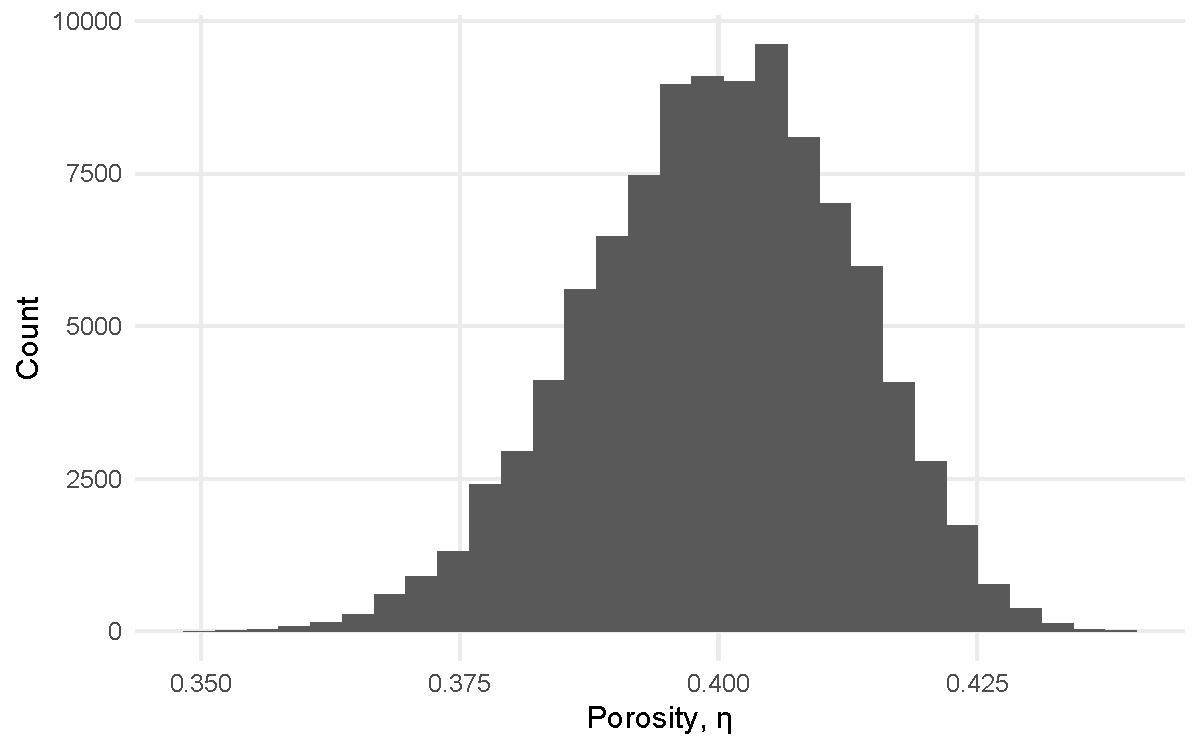
\includegraphics[width=\textwidth]{ch3_appendix_figs/porosity_boot.pdf}
	\caption{Sampling distribution of the porosity sample means from Johnson (1968), Table \ref{ap_b_porosity_boot}. The bootstrapped distribution of 100,000 samples of size n = 5 taken with replacement are approximately normal in distribution. Via the Central Limit Theorem, this indicates that the sampling distribution mean is approximately equal to the population mean. Thus, the sampling distribution mean (0.40) is used as the upscaled porosity in the mixing model. A single value is used because the interquartile range, bounded by 0.39 and 0.41, does not vary appreciably.}
	\label{ap_b_porosity_boot_hist}
\end{figure}

\egroup



%--------------------------------------------------------%
\subsection{Mixing cell model geologic and hydrologic parameters}


% 01_mm_plots_tables.R in F:/ ... POst_QE_Research/DISSERTATION/01_mm
%> c(Williamson, Kang) * 0.3048  # RWI
%[1] 0.243840 0.466055
%> (c(Williamson, Kang) * 0.3048)/2.71232 # divide by 1km unit depth of surface area (SA in km^3)
%[1] 0.0899009 0.1718289


\bgroup

\renewcommand{\arraystretch}{1.5}

\setlength{\tabcolsep}{1.5em}

\begin{table}[H]
	
	\caption{Mixing cell model geologic and hydrologic parameters: $\eta$ is the porosity, $f$ is the aquifer fraction, $\rho$ is the rock-water interaction coefficient, and $E_a$ is the application efficiency. Ranges are provided for parameters used in the Monte Carlo simulation.}
	
	\centering
	
	\begin{tabular}{cccc}
		
		$\bm{\eta \:\: [-]}$ & $\bm{f \:\: [-]}$ & $\bm{\rho \:\: [mg/km^3]}$ & $\bm{E_a \:\: [-]}$\\ 
		\hline
		0.40 & 0.99 & 0.09 - 0.17 & 0.78 - 0.88\\ 
		\hline
	\end{tabular}
	
	\label{ap_b_geometry}
\end{table}

\egroup



%--------------------------------------------------------%
\subsection{Mixing cell model mass balance error}



\bgroup
\setlength{\tabcolsep}{3.5 em}

\centering
\renewcommand{\arraystretch}{1.0}

% 01_mm_plots_tables.R in F:/ ... POst_QE_Research/DISSERTATION/01_mm
% average annual GW budget table - 1961-10-31 to 2001-09-30
% but a lot is added in the caption and table footnote, so beware changing this!!

\begin{threeparttable}
	\begin{table}[H]
		\caption{Cell by cell budget and mass balance error, per equations (9) and (10).}
		
		
		\fontsize{10}{10}\selectfont{
		\begin{tabular}{rlrrrr}
			
			& \textbf{Source} & $\bm{Q \: \: (km^3/yr)}$ &  \\ 
			
			\hline
			\parbox[t]{2mm}{\multirow{7}{*}{\rotatebox[origin=c]{90}{\textbf{j = 1}}}}
			& $N$ & 1.883e+00 \\ 
			& $R$ & 2.451e+00 \\ 
			& $B$ & 2.355e-01 \\ 
			& $M$ & 6.784e-01 \\ 
			& $P_{alt, 1}$ & -3.040e-01 \\ 
			& $q_{1,2}$ & -4.944e+00 \\ 
			& $dS$ & 8.327e-17 \\ 
			\hline  
			\parbox[t]{2mm}{\multirow{5}{*}{\rotatebox[origin=c]{90}{\textbf{j = 2}}}}
			& $q_{1,2}$ & 4.944e+00 \\ 
			& $I_2$ & 6.194e-04 \\ 
			& $P_{alt, 2}$ & -2.864e-01 \\ 
			& $q_{2,3}$ & -4.658e+00 \\ 
			& $dS$ & -2.871e-16 \\ 
			\hline
			\parbox[t]{2mm}{\multirow{5}{*}{\rotatebox[origin=c]{90}{\textbf{j = 3}}}}
			& $q_{2,3}$ & 4.658e+00 \\ 
			& $I_3$ & 5.836e-04 \\ 
			& $P_{alt, 3}$ & -2.698e-01 \\ 
			& $q_{3,4}$ & -4.389e+00 \\ 
			& $dS$ & -1.717e-16 \\ 
			\hline
			\parbox[t]{2mm}{\multirow{5}{*}{\rotatebox[origin=c]{90}{\textbf{j = 4}}}}
			& $q_{3,4}$ & 4.389e+00 \\ 
			& $I_4$ & 5.499e-04 \\ 
			& $P_{alt, 4}$ & -2.542e-01 \\ 
			& $q_{4,5}$ & -4.135e+00 \\ 
			& $dS$ & 8.587e-17 \\ 
			\hline
			\parbox[t]{2mm}{\multirow{5}{*}{\rotatebox[origin=c]{90}{\textbf{j = 5}}}}
			& $q_{4,5}$ & 4.135e+00 \\ 
			& $I_5$ & 5.181e-04 \\ 
			& $P_{alt, 5}$ & -2.395e-01 \\ 
			& $q_{5,6}$ & -3.896e+00 \\ 
			& $dS$ & 2.676e-16 \\ 
			\hline
			\parbox[t]{2mm}{\multirow{5}{*}{\rotatebox[origin=c]{90}{\textbf{j = 6}}}}
			& $q_{5,6}$ & 3.896e+00 \\ 
			& $I_6$ & 4.882e-04 \\ 
			& $P_{alt, 6}$ & -2.257e-01 \\ 
			& $q_{6,7}$ & -3.671e+00 \\ 
			& $dS$ & -4.636e-16 \\ 
			\hline
			\parbox[t]{2mm}{\multirow{5}{*}{\rotatebox[origin=c]{90}{\textbf{j = 7}}}}
			& $q_{6,7}$ & 3.671e+00 \\ 
			& $I_7$ & 4.599e-04 \\ 
			& $P_{alt, 7}$ & -2.126e-01 \\ 
			& $q_{7,8}$ & -3.459e+00 \\ 
			& $dS$ & 1.494e-16 \\ 
			\hline
			\parbox[t]{2mm}{\multirow{5}{*}{\rotatebox[origin=c]{90}{\textbf{j = 8}}}}
			& $q_{7,8}$ & 3.459e+00 \\ 
			& $I_8$ & 7.498e-03 \\ 
			& $P_{alt, 8}$ & -3.466e+00 \\ 
			& $q_{8,9}$ & -6.250e-16 \\ 
			& $dS$ & -3.691e-16 \\ 
			\hline
			
		\end{tabular}
	}
		Cell by cell groundwater flows (Figure 3) are in steady state ($dS \approx MB_{error, j} \approx 0$). $N$ enters the top of the groundwater mixing cell model along with recharge from streams, lakes, and watersheds ($R$), boundary inflow from mountain front recharge ($B$), and managed aquifer recharge ($M$). Subsidence flow $C_{alt}$ = 0, per equation (\ref{eq: p_alt}). Subsurface inflow from the north ($I$) and pumping ($P$) are distributed proportional to cell volume ($V_j$). 
		
		\label{ap_b_cbc}
	\end{table}
	
\end{threeparttable}

\egroup




% body of table is in MCMM_no_RWI_2.Rmd 
% print(xtable(t3), tabluar.environment = "longtable", include.rownames = FALSE)
% longtable example: http://users.sdsc.edu/~ssmallen/latex/longtable.html

\bgroup

\renewcommand{\arraystretch}{1.1}

\setlength{\tabcolsep}{1.0em}

\begin{table}[H]
	\caption{Mixing model TDS-depth profile over time. Median and IQR refer to the median and interquartile range of TDS ($mg/L$) at the depth ($d$) of the cell bottom.}
	\centering
	\fontsize{12}{10}\selectfont{
		\begin{tabular}{@{\extracolsep{2 pt}}llllll@{}}
			
			&  & \multicolumn{2}{c}{\textbf{No RWI}} &  \multicolumn{2}{c}{\textbf{RWI present}}    \\ 
			\cline{3-4} \cline{5-6} \\ 
			$\bm{t \: (yrs)}$ & $\bm{d \: (m)}$ & \textbf{Median} & \textbf{IQR} &  \textbf{Median} & \textbf{IQR} \\ 
			\hline 
			
			\hline
			0 & 36 & 506 & 506-506 & 506 & 506-506 \\ 
			50 & 36 & 975 & 871-1124 & 1111 & 1007-1265 \\ 
			100 & 36 & 1101 & 961-1310 & 1369 & 1208-1603 \\ 
			150 & 36 & 1204 & 1029-1473 & 1600 & 1384-1922 \\ 
			200 & 36 & 1314 & 1100-1654 & 1836 & 1558-2264 \\ 
			250 & 36 & 1434 & 1176-1861 & 2081 & 1733-2638 \\ 
			300 & 36 & 1574 & 1264-2103 & 2345 & 1915-3057 \\ 
			\hline
			0 & 70 & 543 & 543-543 & 543 & 543-543 \\ 
			50 & 70 & 543 & 543-543 & 672 & 650-693 \\ 
			100 & 70 & 960 & 865-1094 & 1218 & 1128-1361 \\ 
			150 & 70 & 1113 & 977-1315 & 1493 & 1346-1729 \\ 
			200 & 70 & 1218 & 1047-1480 & 1717 & 1518-2045 \\ 
			250 & 70 & 1326 & 1116-1659 & 1945 & 1688-2383 \\ 
			300 & 70 & 1449 & 1195-1867 & 2188 & 1864-2743 \\ 
			\hline
			0 & 102 & 571 & 571-571 & 571 & 571-571 \\ 
			50 & 102 & 571 & 571-571 & 692 & 672-712 \\ 
			100 & 102 & 571 & 571-571 & 813 & 773-853 \\ 
			150 & 102 & 948 & 863-1070 & 1320 & 1231-1451 \\ 
			200 & 102 & 1120 & 988-1314 & 1606 & 1463-1830 \\ 
			250 & 102 & 1230 & 1063-1486 & 1829 & 1637-2144 \\ 
			300 & 102 & 1342 & 1136-1667 & 2056 & 1807-2485 \\ 
			\hline
			0 & 132 & 609 & 609-609 & 609 & 609-609 \\ 
			50 & 132 & 609 & 609-609 & 723 & 704-742 \\ 
			100 & 132 & 609 & 609-609 & 837 & 798-874 \\ 
			150 & 132 & 609 & 609-609 & 950 & 893-1007 \\ 
			200 & 132 & 938 & 861-1048 & 1409 & 1317-1532 \\ 
			250 & 132 & 1124 & 997-1310 & 1705 & 1565-1923 \\ 
			300 & 132 & 1245 & 1082-1494 & 1934 & 1742-2243 \\ 
			\hline
			0 & 160 & 637 & 637-637 & 637 & 637-637 \\ 
			50 & 160 & 637 & 637-637 & 744 & 726-762 \\ 
			100 & 160 & 637 & 637-637 & 851 & 816-887 \\ 
			150 & 160 & 637 & 637-637 & 959 & 905-1012 \\ 
			200 & 160 & 637 & 637-637 & 1066 & 994-1137 \\ 
			250 & 160 & 931 & 861-1030 & 1493 & 1388-1599 \\ 
			300 & 160 & 1131 & 1010-1308 & 1793 & 1650-2006 \\ 
			\hline
			0 & 187 & 656 & 656-656 & 656 & 656-656 \\ 
			50 & 187 & 656 & 656-656 & 757 & 740-773 \\ 
			100 & 187 & 656 & 656-656 & 858 & 824-891 \\ 
			150 & 187 & 656 & 656-656 & 959 & 908-1009 \\ 
			200 & 187 & 656 & 656-656 & 1060 & 992-1127 \\ 
			250 & 187 & 656 & 656-656 & 1161 & 1076-1245 \\ 
			300 & 187 & 930 & 867-1020 & 1562 & 1450-1670 \\ 
			\hline
			0 & 212 & 684 & 684-684 & 684 & 684-684 \\ 
			50 & 212 & 684 & 684-684 & 779 & 763-795 \\ 
			100 & 212 & 684 & 684-684 & 874 & 842-906 \\ 
			150 & 212 & 684 & 684-684 & 969 & 922-1017 \\ 
			200 & 212 & 684 & 684-684 & 1065 & 1001-1128 \\ 
			250 & 212 & 684 & 684-684 & 1160 & 1080-1239 \\ 
			300 & 212 & 684 & 684-684 & 1255 & 1159-1350 \\
			\hline
			
		\end{tabular}
	}
	\label{ap_b_p_sim}
\end{table}



% run for M with TDS = 0 mg/L  
% in MCMM.R change:
% annual_fluxes$TDS = c(0,gwc,gwc,gwc,gwc,gwc,0,gwc,0,gwc)
% to:
% annual_fluxes$TDS = c(0,gwc,gwc,gwc,gwc,gwc,0,gwc,0,0)
% Note the final value in the vector is the TDS of M, and changes from the gw concentration (104.6 mg/L) to 0 mg/L.

\bgroup

\renewcommand{\arraystretch}{1.1}

\setlength{\tabcolsep}{1.0em}

\begin{table}[H]
	\caption{Mixing model TDS-depth profile over time when the TDS of $M$ = 0 $mg/L$. Median and IQR refer to the median and interquartile range of TDS ($mg/L$) at the depth ($d$) of the cell bottom.}
	\centering
	\fontsize{12}{10}\selectfont{
		\begin{tabular}{@{\extracolsep{2 pt}}llllll@{}}
			
			&  & \multicolumn{2}{c}{\textbf{No RWI}} &  \multicolumn{2}{c}{\textbf{RWI present}}    \\ 
			\cline{3-4} \cline{5-6} \\ 
			$\bm{t \: (yrs)}$ & $\bm{d \: (m)}$ & \textbf{Median} & \textbf{IQR} &  \textbf{Median} & \textbf{IQR} \\ 
			\hline 
			
			\hline
			0 & 36 & 506 & 506-506 & 506 & 506-506 \\ 
			50 & 36 & 963 & 859-1112 & 1099 & 995-1252 \\ 
			100 & 36 & 1086 & 945-1294 & 1354 & 1193-1587 \\ 
			150 & 36 & 1186 & 1012-1454 & 1582 & 1367-1903 \\ 
			200 & 36 & 1292 & 1080-1631 & 1814 & 1538-2241 \\ 
			250 & 36 & 1410 & 1153-1833 & 2057 & 1710-2611 \\ 
			300 & 36 & 1546 & 1238-2071 & 2317 & 1889-3026 \\ 
			\hline
			0 & 70 & 543 & 543-543 & 543 & 543-543 \\ 
			50 & 70 & 543 & 543-543 & 672 & 650-693 \\ 
			100 & 70 & 949 & 854-1083 & 1207 & 1117-1350 \\ 
			150 & 70 & 1098 & 962-1299 & 1478 & 1332-1713 \\ 
			200 & 70 & 1200 & 1030-1462 & 1699 & 1501-2026 \\ 
			250 & 70 & 1305 & 1096-1636 & 1923 & 1668-2361 \\ 
			300 & 70 & 1425 & 1173-1840 & 2163 & 1842-2717 \\ 
			\hline
			0 & 102 & 571 & 571-571 & 571 & 571-571 \\ 
			50 & 102 & 571 & 571-571 & 692 & 672-712 \\ 
			100 & 102 & 571 & 571-571 & 813 & 773-853 \\ 
			150 & 102 & 938 & 853-1060 & 1310 & 1221-1441 \\ 
			200 & 102 & 1105 & 974-1299 & 1591 & 1449-1815 \\ 
			250 & 102 & 1212 & 1045-1467 & 1811 & 1620-2126 \\ 
			300 & 102 & 1321 & 1117-1645 & 2035 & 1788-2462 \\ 
			\hline
			0 & 132 & 609 & 609-609 & 609 & 609-609 \\ 
			50 & 132 & 609 & 609-609 & 723 & 704-742 \\ 
			100 & 132 & 609 & 609-609 & 837 & 798-874 \\ 
			150 & 132 & 609 & 609-609 & 950 & 893-1007 \\ 
			200 & 132 & 929 & 852-1039 & 1400 & 1308-1523 \\ 
			250 & 132 & 1110 & 984-1295 & 1690 & 1551-1909 \\ 
			300 & 132 & 1228 & 1065-1476 & 1917 & 1725-2225 \\ 
			\hline
			0 & 160 & 637 & 637-637 & 637 & 637-637 \\ 
			50 & 160 & 637 & 637-637 & 744 & 726-762 \\ 
			100 & 160 & 637 & 637-637 & 851 & 816-887 \\ 
			150 & 160 & 637 & 637-637 & 959 & 905-1012 \\ 
			200 & 160 & 637 & 637-637 & 1066 & 994-1137 \\ 
			250 & 160 & 922 & 853-1022 & 1485 & 1380-1591 \\ 
			300 & 160 & 1117 & 996-1294 & 1779 & 1637-1992 \\ 
			\hline
			0 & 187 & 656 & 656-656 & 656 & 656-656 \\ 
			50 & 187 & 656 & 656-656 & 757 & 740-773 \\ 
			100 & 187 & 656 & 656-656 & 858 & 824-891 \\ 
			150 & 187 & 656 & 656-656 & 959 & 908-1009 \\ 
			200 & 187 & 656 & 656-656 & 1060 & 992-1127 \\ 
			250 & 187 & 656 & 656-656 & 1161 & 1076-1245 \\ 
			300 & 187 & 922 & 859-1013 & 1554 & 1442-1663 \\ 
			\hline
			0 & 212 & 684 & 684-684 & 684 & 684-684 \\ 
			50 & 212 & 684 & 684-684 & 779 & 763-795 \\ 
			100 & 212 & 684 & 684-684 & 874 & 842-906 \\ 
			150 & 212 & 684 & 684-684 & 969 & 922-1017 \\ 
			200 & 212 & 684 & 684-684 & 1065 & 1001-1128 \\ 
			250 & 212 & 684 & 684-684 & 1160 & 1080-1239 \\ 
			300 & 212 & 684 & 684-684 & 1255 & 1159-1350 \\ 
			\hline
			
		\end{tabular}
	}
	\label{ap_b_p_sim_m_with_tds_0}
\end{table}


\clearpage



%--------------------------------------------------------%
% Acknowledgments
%--------------------------------------------------------%
\section{Acknowledgments}

We gratefully thank Drs. Helen Dahlke, Jonathan Herman, Randy Dahlgren, Laura Foglia, and Yong Zhang for their feedback and modeling advice. Dr. Can Dogrul and the California Department of Water Resources Groundwater Modeling division offered instrumental C2VSim modeling guidance. Support for this research was provided by the University of California Agricultural and Natural Resources grant CA-D-LAW-6036-H, the National Science Foundation (NSF) Climate Change, Water, and Society (CCWAS) Integrated Graduate Education and Research Traineeship (IGERT) program at the University of California, Davis (http://ccwas.ucdavis.edu, DGE-10693333), the U.S./China Clean Energy Research Center for Water-Energy Technologies (CERC-WET), and
the UC Office of the President’s Multi-Campus Research Programs and
Initiatives (MR-15-328473) through UC Water, the University of
California Water Security and Sustainability Research Initiative. All data is accessible via Dryad at \textit{https://datadryad.org/stash/dataset/doi:10.25338/B81P5K}, and procedures and models are accessible at \textit{https://github.com/richpauloo/Monte-Carlo-Mixing-Model} \citep{Pauloo2020}.  

\clearpage